% !TeX spellcheck = en_GB
%%%%%%%%%%%%%%%%%%%%%%%%%%%%%%%%%%%%%%%%%%%%%%%%%%%%%%%%%%%%%%%%%%%%%%%%%%%%%%%%
%2345678901234567890123456789012345678901234567890123456789012345678901234567890
%        1         2         3         4         5         6         7         8

\documentclass[letterpaper, 10 pt, conference]{ieeeconf}  % Comment this line out if you need a4paper

%\documentclass[a4paper, 10pt, conference]{ieeeconf}      % Use this line for a4 paper

\IEEEoverridecommandlockouts                              % This command is only needed if 
                                                          % you want to use the \thanks command

\overrideIEEEmargins                                      % Needed to meet printer requirements.

% See the \addtolength command later in the file to balance the column lengths
% on the last page of the document

% The following packages can be found on http:\\www.ctan.org
%\usepackage{graphics} % for pdf, bitmapped graphics files
%\usepackage{epsfig} % for postscript graphics files
%\usepackage{mathptmx} % assumes new font selection scheme installed
%\usepackage{times} % assumes new font selection scheme installed
\usepackage{float}
\usepackage{ngerman}
\usepackage[utf8]{inputenc}
\usepackage{color, colortbl}
\usepackage{amsmath}
%\usepackage{bm}
\newcommand{\bm}[1]{\boldsymbol{#1}}
\usepackage{amssymb}
\usepackage{todonotes}
\usepackage{graphicx}
\graphicspath{{./figures/}}
% Symbole für Tabelle: grüner Haken und rotes Kreuz
\newcommand{\ok}{{\color{green}\checkmark}}
\newcommand{\no}{{\color{red}$\boldsymbol\times$}}

\definecolor{Gray}{gray}{0.9}
\definecolor{LightCyan}{rgb}{0.88,1,1}

\usepackage{calrsfs}
\DeclareMathAlphabet{\pazocal}{OMS}{zplm}{m}{n}
\newcommand{\body}[1]{\mathcal{B}_{#1}}
\newcommand{\ks}[1]{\mathcal{F}_{#1}}
\newcommand{\cc}[1]{\mathcal{C}_{#1}}
\newcommand{\ortvek}[3]{{ }_{(#1)}{\boldsymbol{r}}^{#2}_{#3}}
\renewcommand{\vec}[1]{\mbox{\boldmath{$#1$}}}
\newcommand{\tmat}[2]{{^{\mathrm{#1}}\vec{T}_{\mathrm{#2}}}}

% Markup package
\usepackage[deletedmarkup=xout,authormarkup=none]{changes}
\setremarkmarkup{\emph{(#1: #2)}}
\colorlet{lg}{red!80!black}
\colorlet{sp}{blue!80!black}
%\setremarkmarkup{\emph{\color{lg!70!white}\small(#1: #2)}}
\definechangesauthor[color=lg]{Lg}
\definechangesauthor[color=sp]{Sp}

% Geometrische Bezeichnungen des Mechanismus. Sind in schriftlichen Aufzeichnungen nicht konsistent. Daher wird die Benennung in diesem Paper geändert. Zur Übersichtlichkeit werden die alten Bezeichnungen als Makro verwendet.
% https://tex.stackexchange.com/a/9728
\makeatletter
\newcommand{\gdelta}{\afterassignment\gdelta@aux\count0=}
\newcommand{\gdelta@aux}{\csname gdelta\the\count0\endcsname}
\newcommand{\gdotdelta}{\afterassignment\gdotdelta@aux\count0=}
\newcommand{\gdotdelta@aux}{\csname gdotdelta\the\count0\endcsname}
\newcommand{\ggamma}{\afterassignment\ggamma@aux\count0=}
\newcommand{\ggamma@aux}{\csname ggamma\the\count0\endcsname}
\newcommand{\gbeta}{\afterassignment\gbeta@aux\count0=}
\newcommand{\gbeta@aux}{\csname gbeta\the\count0\endcsname}
\newcommand{\gl}{\afterassignment\gl@aux\count0=}
\newcommand{\gl@aux}{\csname gl\the\count0\endcsname}
\newcommand{\ghl}{\afterassignment\ghl@aux\count0=}
\newcommand{\ghl@aux}{\csname ghl\the\count0\endcsname}
\makeatother

\newif\ifneuenomenklatur
\neuenomenklaturtrue

% Neue Bezeichnungen:
\ifneuenomenklatur
    \expandafter\newcommand\csname gdelta8\endcsname{%
        \eta_1}
    \expandafter\newcommand\csname gdelta6\endcsname{%
        \eta_2}
    \expandafter\newcommand\csname gdelta16\endcsname{%
        \eta_3}
    \expandafter\newcommand\csname gdelta3\endcsname{%
        \eta_4}
    \expandafter\newcommand\csname gdelta19\endcsname{%
        \eta_5}
    \expandafter\newcommand\csname gdotdelta19\endcsname{%
        \dot{\eta}_5}
    \expandafter\newcommand\csname gdelta17\endcsname{%
        \eta_6}
    \expandafter\newcommand\csname gbeta1\endcsname{%
        \eta_7}
    \expandafter\newcommand\csname gdelta18\endcsname{%
        \eta_8}
    \expandafter\newcommand\csname ggamma5\endcsname{%
        \eta_9}
    \expandafter\newcommand\csname ggamma3\endcsname{%
        \eta_{10}}
    \expandafter\newcommand\csname gdelta7\endcsname{%
        \eta_{11}}
    \expandafter\newcommand\csname gdelta9\endcsname{%
        \eta_{12}}
    \expandafter\newcommand\csname gdelta20\endcsname{%
        \eta_{13}}
    \expandafter\newcommand\csname gl1\endcsname{%
        L_1}
    \expandafter\newcommand\csname gl2\endcsname{%
        L_2}
    \expandafter\newcommand\csname gl3\endcsname{%
        L_3}
    \expandafter\newcommand\csname gl4\endcsname{%
        L_8}
    \expandafter\newcommand\csname gl5\endcsname{%
        L_4}
    \expandafter\newcommand\csname gl6\endcsname{%
        L_9}
    \expandafter\newcommand\csname gl11\endcsname{%
        2L_5}
    \expandafter\newcommand\csname ghl11\endcsname{%
        L_5}
    \expandafter\newcommand\csname gl12\endcsname{%
        2L_6}
    \expandafter\newcommand\csname ghl12\endcsname{%
        L_6}
    \expandafter\newcommand\csname gl13\endcsname{%
        L_{13}}
    \expandafter\newcommand\csname gl14\endcsname{%
        L_{11}}
    \expandafter\newcommand\csname gl15\endcsname{%
        L_7}
    \expandafter\newcommand\csname gl20\endcsname{%
        L_{12}}
    \expandafter\newcommand\csname gl21\endcsname{%
        L_{14}}
    \expandafter\newcommand\csname gl22\endcsname{%
        L_{10}}
    \expandafter\newcommand\csname gl16\endcsname{%
        L_\mathrm{s}}
\else
    % Original-Bezeichnungen:
    \expandafter\newcommand\csname gdelta8\endcsname{%
        \delta_8}
    \expandafter\newcommand\csname gdelta6\endcsname{%
        \delta_6}
    \expandafter\newcommand\csname gdelta16\endcsname{%
        \delta_{16}}
    \expandafter\newcommand\csname gdelta3\endcsname{%
        \delta_3}
    \expandafter\newcommand\csname gdelta19\endcsname{%
        \delta_{19}}
    \expandafter\newcommand\csname gdotdelta19\endcsname{%
        \dot{\delta}_{19}}
    \expandafter\newcommand\csname gdelta17\endcsname{%
        \delta_{17}}
    \expandafter\newcommand\csname gbeta1\endcsname{%
        \beta_1}
    \expandafter\newcommand\csname gdelta18\endcsname{%
        \delta_{18}}
    \expandafter\newcommand\csname ggamma5\endcsname{%
        \gamma_5}
    \expandafter\newcommand\csname ggamma3\endcsname{%
        \gamma_3}
    \expandafter\newcommand\csname gdelta7\endcsname{%
        \delta_7}
    \expandafter\newcommand\csname gdelta9\endcsname{%
        \delta_9}
    \expandafter\newcommand\csname gdelta20\endcsname{%
        \delta_{20}}
    \expandafter\newcommand\csname gl1\endcsname{%
        l_1}
    \expandafter\newcommand\csname gl2\endcsname{%
        l_2}
    \expandafter\newcommand\csname gl3\endcsname{%
        l_3}
    \expandafter\newcommand\csname gl4\endcsname{%
        l_4}
    \expandafter\newcommand\csname gl5\endcsname{%
        l_5}
    \expandafter\newcommand\csname gl6\endcsname{%
        l_6}
    \expandafter\newcommand\csname gl11\endcsname{%
        l_{11}}
    \expandafter\newcommand\csname ghl11\endcsname{%
        l_{11}/2}
    \expandafter\newcommand\csname gl12\endcsname{%
        l_{12}}
    \expandafter\newcommand\csname ghl12\endcsname{%
        l_{12}/2}
    \expandafter\newcommand\csname gl13\endcsname{%
        l_{13}}
    \expandafter\newcommand\csname gl14\endcsname{%
        l_{14}}
    \expandafter\newcommand\csname gl15\endcsname{%
        l_{15}}
    \expandafter\newcommand\csname gl20\endcsname{%
        l_{20}}
    \expandafter\newcommand\csname gl21\endcsname{%
        l_{21}}
    \expandafter\newcommand\csname gl22\endcsname{%
        l_{22}}
    \expandafter\newcommand\csname gl16\endcsname{%
        l_\mathrm{F}}
\fi

\title{\LARGE \bf
Kinematics and Dynamics Model via Explicit Trigonometric Elimination of Kinematic Constraints for a Force Assistance Exoskeleton
}


\author{Moritz Schappler$^{1}$ and Sami Haddadin$^{2}$% <-this % stops a space
\thanks{*This work was supported by the German Federal Ministry of Education and Research (BMBF) under grant no. 16SV6175.}% <-this % stops a space
\thanks{$^{1}$Moritz Schappler
        {\tt\small schappler@imes.uni-hannover.de}}%
\thanks{$^{2}$Sami Haddadin
        {\tt\small sami.haddadin@tum.de}}%
}


\begin{document}



\maketitle
\thispagestyle{empty}
\pagestyle{empty}


%%%%%%%%%%%%%%%%%%%%%%%%%%%%%%%%%%%%%%%%%%%%%%%%%%%%%%%%%%%%%%%%%%%%%%%%%%%%%%%%
\begin{abstract}

The efficient implementation of kinematics and dynamics models is a key to model based control of mechatronic systems such as robots and wearable assistive devices.
This paper presents an approach for the derivation of these models in symbolic form based on the explicit elimination of the kinematic constraints using substitution variables with trigonometric expressions and the Lagrange equations of the second kind.
This represents an alternative solution to using the implicit form of the constraints or using the explicit elimination with comparable computational effort.
%
The method is applied on an exoskeleton designed for craftsmen force assistance, which consists of multiple planar closed kinematic loops and gear mechanisms.

\end{abstract}

%%%%%%%%%%%%%%%%%%%%%%%%%%%%%%%%%%%%%%%%%%%%%%%%%%%%%%%%%%%%%%%%%%%%%%%%%%%%%%%%
\section{Introduction and State of the Art}

%Die Einsatzgebiete körpergetragene Systeme teilen sich u.a. auf in Exoskelette zur Rehabilitation und Kraftunterstützung, haptische Eingabegeräte und Prothesen.
%Exoskelette werden körpernah getragen und verlaufen in ihrer Gelenkstruktur parallel zu den menschlichen Gliedmaßen.
%Daher müssen die Gelenke des Mechanismus die Freiheitsgrade der Gelenke des Menschen nicht beschränken, um Zwangskräfte zu vermeiden, die dauerhaft zu Diskomfort und gesundheitlicher Schädigung führen.
Body mounted robotic systems are an increasing field of research to encounter the challenges of augmenting the humans capabilities\added[id=Lg]{, especially when facing the demographic change}.
The domain can be clustered in exoskeletons for rehabilitation and force assistance, devices for human-machine-interaction and telepresence and prostheses.
Exoskeletons are aligned close to the human body along the structure of the human limbs and joints.
Constraining the human joint movements results in constraint forces leading to discomfort and long-term wear \cite{Pons2008}.
%
%Die Mechanismen für Exoskelette verfügen daher über mehr Gelenke als klassische Industrieroboter mit derselben Zahl an Freiheitsgraden.
Therefore exoskeleton mechanisms usually have more degrees of freedom (DoF) than classical robots with the same number of end-effector DoF.

%Zusätzlich müssen Je nach Szenario nicht alle Bewegungsrichtungen aktuiert werden.
%Während Rehabilitations-Exoskelette je nach Einschränkung des Patienten mehr Führung bieten, ist bei Kraftunterstützungssystemen hauptsächlich eine Unterstützung in Gravitationsrichtung notwendig.

Depending on the application area not all directions of motion have to be actuated.
While exoskeletons for rehabilitation provide more guidance to the user depending on the impairment of the patient, force assistance exoskeletons mainly need to assist in the direction of gravity.
%
%%ESA Space robotics telepresence exoskeleton \cite{SchieleVis2003}, 
%
%%Beispiele für Reha-Exos sind z.B. ... 
%%WOTAS für Tremor

Examples for upper limb rehabilitation exoskeletons are the WOTAS exoskeleton for tremor suppression \cite{RoconBelRuiMan2007} and the shoulder rehabilitation exoskeleton from Carignan et al. \cite{CarignanLis2005}.

%Kraftunterstützungs-Exos z.B. ...
Known exoskeletons for force assistance are among others the Bleex lower limb exoskeleton \cite{ChuKazZos2005} and the HAL \cite{Sankai2010} and Raytheon XOS upper and lower body exoskeleton as well as the upper limb exoskeletons from Hsieh et al. \cite{HsiehChiLan2015}. 
The Fraunhofer upper limbs Exo-Jacket \cite{Ebrahimi2017} and full-body exoskeleton Robo-Mate \cite{StadlerAltSchSch2017} are systems designed for the use in industrial scenarios.

%Da die Systeme oftmals erst durch eine modellbasierte Regelung ein gutes Nutzerverhalten z.B. durch Impedanz- oder Kraftregelung erhalten, ist eine effiziente Modellierung dieser Systeme mit in Echtzeit ausführbaren Modellen  höchst relevant.
Since a good user experience of these active systems is often only possible with a model-based control like impedance and force control, a computationally efficient model of the system, which has to run in real-time, is crucial.


%Modellierung:
%Die mechanische Modellierung der Systeme kann durch ein Starrkörpermodell mit diskreten Gelenken vorgenommen werden.
%Dies kann bei Mechanismen mit flexiblen Elementen wie ... eine erste Näherung darstellen oder bereits eine gute Beschreibung des Verhaltens von Systemen wie ... darstellen.
The mechanics modelling of the systems can be performed with the assumption of rigid bodies and basic joints \cite{Pons2008}.
%For systems with flexible elements this approach can be completely insufficient or with modifications a usable approximation. For other systems this can be a good description of the system behaviour.

%Die Modellierung kann durch die gleichen Methoden wie für Roboter erfolgen, jedoch sind hier passive Freiheitsgrade des Endeffektors vorhanden, die durch den Benutzer ausgeglichen werden.
If this assumption holds, the modelling can be done with the same multi body dynamics methods as for industrial robots.
However unlike in classical robotics, the exoskeleton systems can contain passive end-effector DoF that are levelled out by the user.

%Die Kopplung der Systeme mit dem Nutzer kann zum Einen kinematisch durch Zwangsbedingungen beschrieben werden, dazu ist jedoch eine Schätzung des Nutzerverhaltens wie in ... notwendig.
%Hier wird eine einfachere isolierte Betrachtung des Nutzers durch extern angreifende Kräfte angenommen.
If the coupling of the systems with the user is described kinematically with constraint equations, an estimation of the users pose is necessary.
In this work, an isolated view of the system is taken with the user considered via external forces and moments.
%
%Mechanische Zwangsbedingungen treten dann nur noch im Mechanismus selbst auf, z.B. durch parallele mechanische Strukturen.
With this assumption mechanical constraints may only occur in the mechanism itself, e.\,g. due to closed kinematic loops.

%Die Lösung von kinematischen Zwangsbedingungen für mechanische Systeme kann allgemein durch die implizite Darstellung erfolgen.
%Die Lösung der Dynamikgleichungen kann durch die Invertierung der daraus resultierenden Jacobi-Matrix mit den Lagrange-Gleichungen erster Art [Quelle] oder der Udwadia-Kalaba-Gleichung [Quelle] erfolgen.
%Ersteres ist in den symbolischen Rechenprogrammen Robotran [Quelle] und openSYMORO [Quelle] implementiert.
%Die Jacobi-Matrix der Zwangsbedingungen kann entweder aus der expliziten Form der ZB [Quelle] oder der impliziten Form [Quelle] erfolgen.

The equations of motion of mechanic systems with kinematic constraints can in general be found with the implicit formulation of these constraints.
The dynamics equations can be derived via the inverse of the constraints Jacobian with Lagrange multipliers \cite{NakamuraGho1989} or the Udwadia-Kalaba-equation \cite{UdwadiaKal1992}.
The former is implemented in symbolic multi body algorithms such as Robotran \cite{SaminFis2013} or openSymoro \cite{KhalilVijKhoMuk2014}.
The constraints Jacobian can be either derived from the explicit form of the constraints \cite{NakamuraGho1989} or from the time derivative of the implicit form \cite{ParkChoPlo1999}.

%Für die rechentechnisch effiziente Beschreibung sind symbolisch generierte Modellgleichungen vorteilhaft [Quelle]. Damit sind auch weitere Untersuchungen möglich wie die Gruppierung der Dynamikparameter in der parameterlinearer Form \cite{KhalilBen1995} oder weitere Untersuchungen [Quelle Park?].
For the computationally efficient analysis of mechanisms it is advantageous to derive the equations of motion in symbolic form \cite{SaminFis2013}.
\replaced[id=Lg]{This also facilitates or improves}{Then also} further steps such as grouping dynamics parameters to a minimal set  in the regressor form of the dynamics equations \cite{KhalilBen1995} or aspects such as linearisation, control and optimization\deleted[id=Lg]{ are facilitated or improved} \cite{ParkChoPlo1999}.

%Die explizite Darstellung erfordert eine händische Untersuchung des Mechanismus und ist nur für eine eingeschränkte Klasse von Mechanismen verfügbar während sich die implizite Darstellung für alle Systeme und den Einsatz automatischer Programme eignet. Dieser Ansatz wird daher auch in o.g. CAS standardmäßig eingesetzt

An explicit representation of the constraints often requires manual generation of the expressions and is only possible for a small set of mechanisms, e.\,g. some types of planar closed loops.
The implicit representation is available for all systems and is therefore used in the methods and tools mentioned above.

%Eine analytische Beschreibung aller kinematischer Größen ist nur bei expliziter Berechnung der Zwangsbedingungen möglich. Bei impliziter Berechnung müssen diese numerisch iterativ bestimmt werden.

The direct calculation of all active and passive joint coordinates of a mechanism is only possible with the explicit form of the kinematic constraints.
If only the implicit form is available, dependant coordinates have to be determined with numeric iterative procedures \cite{ParkChoPlo1999}.

%Die Herleitung symbolischer Gleichungen für Kinematik und Dynamik werden in diesem Paper anhand eines Beispielsystems aus der Klasse der Exoskelette untersucht. Dabei wird die explizite Darstellung der Zwangsbedingungen verwendet und die Struktur der Dynamikgleichungen für symbolische Vereinfachungen genutzt.
In this paper, the derivation of symbolic equations for the kinematics and dynamics is demonstrated at the example of an upper limb exoskeleton.
The explicit form of the kinematic constraints is given and the structure of the dynamics equations is used for symbolic simplifications leading to improved computational efficiency.

%
%
%The field of wearable robotic systems aims to 
%Exoskeletons for assistance and rehabilitation
%
%list different upper limb exoskeletons with different concepts
%
%techniques and tools for kinematics and dynamics modelling
%
%model assumptions for wearable robots: kinematic coupling of human and exoskeleton. Exoskeleton may contain passive joints (unlike serial chain robots), floating base assumption for base forces

The contributions of the paper are
\begin{itemize}
    \item the presentation of a novel exoskeleton mechanism,
    \item \added[id=Lg]{a formalism for derivation of related models in symbolic form based on the explicit elimination of the kinematic constraints using substitution variables with trigonometric expressions and the Lagrange equations of the second kind,}
    \item the detailed mathematical description of the kinematic modelling of the mechanisms constraints containing gears and multiple closed loops with
    \item a focus on the implementation of these constraints in \emph{trigonometric explicit form} optimized for symbolic processing with computer algebra systems.
\end{itemize}

The exoskeleton mechanism can be regarded as an example to emphasize the advantage of the proposed approach of explicit trigonometric elimination of kinematic constraints.

Therefore, the paper is structured as follows:
In Sec.\,\ref{sec:exo_scenario} the components of the exoskeleton are briefly presented together with the envisioned scenario of its field of application. In Sec.\,\ref{sec:model} the kinematics and dynamics modelling is presented in detail focussing on the formulation of the explicit constraint equations with substitution variables based on trigonometric expressions.
The Sections \ref{sec:actuation_control} and
\ref{sec:simulation} provide an exemplary concept for the actuation and the control of the system and simulation results to validate the model. Sec.\,\ref{sec:conclusion} concludes the paper.

\section{Exoskeleton and Scenario}
\label{sec:exo_scenario}
\subsection{Scenario}

The exoskeleton presented in this paper is targeted as an assistive device for craftsmen working with power tools like a hand-held power drill.
The system is supposed to provide the basic functions
%
\begin{itemize}
    \item \emph{force assistance} with a body mounted robotic structure compensating the weight of the power tool to reduce fatigue and work-related health problems,
    \item \emph{augmented reality} by projection of relevant data and instructions in the user's working space \cite{NuelleBriTapDem2018},
    \item \emph{guiding} by fusion of measurement data, a haptic interface, adaptive control, and interaction functions.
\end{itemize}
%
%The system was developed in a project \cite{NuelleSchTapLil2017} which 
%The project whi
%
%
%force assistance for craftsmen
%project goals : 
%* reduce fatigue of the worker and work-induced diseases, 
%* increase work quality by projection of additional information (augmented reality, )
%* guiding the user
The system was developed within the project ``Third Arm'' \cite{NuelleSchTapLil2017} which continued the work presented in \cite{PetereitAlbJerSch2012}. 
The waist-carried demonstrator from \cite{PetereitAlbJerSch2012} was tested under aspects of ergonomics and workspace and was not able to meet the requirements for the flexible use in a  craftsmen-scenario on construction sites. Thus the following design concept of an upper limb exoskeleton proximal to the users body was developed by the project consortium.

\subsection{Exoskeleton}

The exoskeleton consists of several parts which will be introduced in short before being studied closer regarding kinematics and dynamics models.

\subsubsection{Main structure following the Human Arm}

With the required attachment at the users upper body and at the hand \replaced[id=Lg]{together}{and} with the demand of neither blocking the users workspace nor sight, the main structure of the exoskeleton follows the arm of the user closely with similar DoF as the human arm.

Fig.\,\ref{fig:KAS5_CAD} shows a CAD model of the complete exoskeleton to be carried in a right-hand configuration.


\begin{figure}[tb!]
    \input{./figures/KAS5_Seitenansicht_beschriftet.pdf_tex}
    \caption{CAD model of the exoskeleton mechanism. This CAD model is copyrighted by Michael Winkler and the BMBF project consortium ``Third Arm''.}
    \label{fig:KAS5_CAD}
\end{figure} 

\subsubsection{Three-Axis Elbow Joint}

The elbow joint of the mechanism is aligned to the axis of rotation of the users elbow.
To reduce constraint forces on the users elbow, the joint consists of three parallel axes\footnote{As e.\,g. also shown in \cite{Pons2008} without the gearing mechanism.} which couple the upper arm and the forearm via a central gear wheel. The mechanism is shown in detail in Fig.\,\ref{fig:EllenbogenSimMech} in different poses.
The lever mechanism connecting the linear spring-damper-system with the elbow is fixed to the central elbow gear.

\begin{figure}[tb!]
    \small
    \input{./figures/KAS6m3_Ellenbogen_beschriftet.pdf_tex}
    \caption{Different poses for the three-axes elbow joint. The rigid bodies are emphasized with different colours and the numbers in circles. The coupling mechanism connecting to the shoulder is left out for clarity. This CAD model is copyrighted by Michael Winkler and the BMBF project consortium ``Third Arm''.}
    \label{fig:EllenbogenSimMech}
\end{figure} 

\subsubsection{Three-Axes Shoulder Joint}

The shoulder joint imitates the degrees of freedom of a simplified model of the human shoulder with three consecutive rotations with perpendicular axes.
The last axis of the shoulder joint corresponding to the shoulder flexion/extension (F/E) is parallel to the axes of the elbow and the coupling mechanism, leaving the greatest part of the joints in one plane to simplify manufacturing and kinematics modeling.

\subsubsection{Coupling Mechanism between Shoulder and Elbow}

The shoulder F/E joint and the elbow joint are coupled via a mechanism consisting of two crank-lever mechanisms.
This removes one degree of freedom of the system and forces the shoulder and first elbow rotation to move on a common trajectory.
With this coupling it is possible to transfer forces from the shoulder to the elbow and therefore move a motor actuating the elbow to the shoulder.
This concept is known from industrial robots with parallelogram structure connecting the second and third link where moving the motor near the second joint reduces the inertia and gravitational load of the system.\added[id=Lg,remark={Is there a reference for this?}]{}

\subsubsection{Spring-Damper System}

The elbow joint is connected via the central gear and a linear spring damper system with the forearm.
These spring systems are known e.\,g. for their use in mountain bike suspension forks.
The spring is transferring the moment created by the weight of the powertool towards the central gear and reduces oscillations originating from processes like drilling.

\section{Kinematics and Dynamics Modelling}
\label{sec:model}

\subsection{Kinematic Model and Coordinate Definition}

All rotational axes of the mechanism are described as single-DoF joints using the modified Denavit-Hartenberg notation \cite{KhalilBen1995} to describe the position and orientation of the frames $\ks{i}$ attached to all rigid bodies $\body{i}$ of the mechanism.
The parameters describing the transformations between these frames are given in Tab.\,\ref{tab:mdh_parameter}.
%
\begin{table}
    \centering
    \setlength\tabcolsep{3pt}
    \caption{Kinematic parameters of the structure.}\par\vspace{-3.5ex}
    \begin{tabular}[t]{|c||c|c||c|c||c|c|c|c|c|}
        \hline
        $i$ & $\mu_i$ & $\sigma_i$ & $\gamma_i$ & $\epsilon_i$ & $\alpha_i$ & $d_i$ & $\theta_i$ & $r_i$ & $a(i)$ \\
        \hline
          &   &   & $\bm{R}_{\mathrm{}z}$ & $\bm{T}_{\mathrm{z}}$  & $\bm{R}_{\mathrm{}x}$  & $\bm{T}_{\mathrm{}x}$  &   $\bm{R}_{\mathrm{}z}$ & $ \bm{T}_{\mathrm{z}}$  &   \\
        \hline
        1 & $1$ & $0$ & $0$ & $0$ & $0$ & $0$ & $\rho_1-\pi/2$ & $\gl1$ & 0 \\
        2 & $1$ & $0$ & $0$ & $0$ & $-\pi/2$ & $0$ & $\rho_2+\pi/2$ & $\gl2$ & 1 \\
        3 & $0$ & $0$ & $0$ & $0$ & $\pi/2$ & $0$ & $\rho_3$ & $\gl3$ & 2 \\
        4 & $1$ & $0$ & $0$ & $0$ & $0$ & $\gl5$ & $\rho_4$ & $0$ & 3 \\
        5 & $1$ & $0$ & $0$ & $0$ & $0$ & $\gl11$ & $\rho_5$ & $0$ & 4 \\
        6 & $0$ & $0$ & $0$ & $0$ & $0$ & $\gl12$ & $\rho_6 + \pi/2$ & $0$ & 5 \\
        7 & $1$ & $0$ & $0$ & $0$ & $\pi/2$ & $0$ & $\rho_7$ & $\gl15$ & 6 \\
        8 & $0$ & $2$ & $0$ & $0$ & $\pi/2$ & $0$ & $\gdelta8+\pi/2$ & $\gl3$ & 2 \\
        9 & $0$ & $0$ & $0$ & $0$ & $0$ & $-\gl4$ & $-\gdelta6$ & $0$ & 8 \\
        10 & $0$ & $0$ & $0$ & $0$ & $0$ & $\gl6$ & $-\gdelta16$ & $0$ & 3 \\
        11 & $0$ & $0$ & $0$ & $0$ & $0$ & $\gl22$ & $\pi-\gdelta3$ & $0$ & 10 \\
        12 & $0$ & $0$ & $0$ & $0$ & $0$ & $\gl11$ & $\gdelta19-\pi/2$ & $0$ & 4 \\
        13 & $0$ & $2$ & $0$ & $0$ & $0$ & $0$ & $\gdelta17-\pi/2$ & $0$ & 12 \\
        14 & $0$ & $0$ & $0$ & $0$ & $0$ & $\gl14$ & $3\pi/2-\gbeta1$ & $0$ & 13 \\
        15 & $0$ & $1$ & $0$ & $0$ & $\pi/2$ & $0$ & $0$ & $\gl16$ & 14 \\
        \rowcolor{LightCyan}
        16 & $0$ & $0$ & $\gdelta9$ & $0$ & $0$ & $\gl21$ & $*$ & $0$ & 10 \\
        \rowcolor{LightCyan}
        17 & $0$ & $0$ & $0$ & $0$ & $0$ & $\gl14$ & $*$ & $0$ & 13 \\
        \rowcolor{LightCyan}
        18 & $0$ & $0$ & $-\pi/2-\gdelta20$ & $0$ & $0$ & $\gl22$ & $*$ & $0$ & 6 \\
        \rowcolor{Gray}
        19 & $2$ & $0$ & $0$ & $\gl20$ & $0$ & $0$ & $0$ & $0$ & 9 \\
        \rowcolor{Gray}
        20 & $2$ & $0$ & $0$ & $\gl13$ & $0$ & $0$ & $0$ & $0$ & 11 \\
        \rowcolor{Gray}
        21 & $2$ & $0$ & $-\pi/2$ & $0$ & $0$ & $0$ & $0$ & $0$ & 15 \\
        \hline
    \end{tabular}
    \label{tab:mdh_parameter}
\end{table}
%
\deleted[id=Lg]{A kinematic sketch of the whole mechanism from Fig.\,\ref{fig:KAS5_CAD} is given in Fig.\,\ref{fig:KAS5_kinematik} with annotations for frames, bodies and coordinates according to Tab.\,\ref{tab:mdh_parameter}.}
%
\begin{figure}[tb]
    \begin{center}
        \vspace{0.2cm} % wird für bounding box des Bilds benötigt
        \fontsize{8}{8}\selectfont
        \scalebox{1.15}{\input{./figures/KAS5_m3_skizze_kinematik_2_KS.pdf_tex}}
    \end{center}
    \caption{Kinematic sketch of the mechanism with frames according to Tab.\,\ref{tab:mdh_parameter}. Body numbers are indicated with circles.}
    \label{fig:KAS5_kinematik}
\end{figure}

Due to the structure of the mechanism, the extended notation with anteceding link index $a(i)$, joint type marker $\sigma_i$ (0 for rotational joint, 1 for prismatic joint, 2 for fixed connection) and actuation marker $\mu_i$ (0 for passive, 1 for active joint) is used.
The marker $\mu_i$ is set to 1 for the joints representing the generalized coordinates from (\ref{equ:mincoord}), regardless whether they are actuated or not.
The order of rotations $\bm{R}$ and translations $\bm{T}$ is given in the head row for $\gamma_i$ to $r_i$.
Only the rows 1 to 15 of the table mark frames associated with rigid bodies.
The rows 16-18 denote the first frame and the rows 19-21 the second frame of the cut joints belonging to the three closed kinematic loops.
\added[id=Lg]{A kinematic sketch of the whole mechanism from Fig.\,\ref{fig:KAS5_CAD} is given in Fig.\,\ref{fig:KAS5_kinematik} with annotations for frames, bodies and coordinates according to Tab.\,\ref{tab:mdh_parameter}.}

The mechanism is regarded without the kinematic constraints by virtually cutting the loop-closing joints resulting in a tree structure \cite{KhalilBen1995} and removing the other constraints that are referred to as ``user constraints'' in \cite{SaminFis2013}.
\added[id=Lg]{The joint coordinates of the main structure are denoted with $\rho$ and the coordinates of the parallel coupling and support mechanism with $\eta$.}
\replaced[id=Lg]{According to \cite{NakamuraGho1989}, the}{The} coordinates 
%
\begin{equation}
\bm{q}=\begin{pmatrix}\bm{q}_1^\mathrm{T} & \bm{q}_2^\mathrm{T} \end{pmatrix}^\mathrm{T}
\end{equation}
%
of the single-DoF joints of this unconstrained system can \deleted[id=Lg]{according to \cite{NakamuraGho1989}} be separated into the generalized coordinates
%
\begin{equation}
\bm{q}_1=\begin{pmatrix}\rho_1 & \rho_2 & \rho_4 & \rho_5 &\rho_7 \end{pmatrix}^\mathrm{T}
\label{equ:mincoord}
\end{equation}
%
and the dependent coordinates
%
\begin{equation}
\bm{q}_2=\begin{pmatrix}\rho_3 & \rho_6 & \gdelta6 & \gdelta16 & \gdelta3 & \gdelta19 & \gbeta1 & \gl16 \end{pmatrix}^\mathrm{T}.
\label{equ:depcoord}
\end{equation}
%
The constant kinematics parameters can be grouped in a separate vector
%
\begin{equation}
\bm{p}_\mathrm{kin}=\begin{pmatrix}\gdelta8 & \gdelta17 & \gl1 & \gl2 & ... & \gl13 \end{pmatrix}^\mathrm{T}.
\label{equ:kinparam}
\end{equation}
\added[id=Lg,remark={Is it intended that some $\eta_i$ are parameters and some $L_i$ are dependant coordinates? This might be confusing. Can this be avoided by other namings?}]{}

\replaced[id=Lg]{Without loss of generality, the coordinates $\rho$ and $\eta$ can}{The joint coordinates of the main structure are denoted with $\rho$ and the coordinates of the parallel coupling and support mechanism with $\eta$. These can without loss of generality} be grouped according to the joint type into rotational coordinates $\bm{q}_{\mathrm{R}}$ corresponding to $\sigma_i=0$ and translational coordinates $\bm{q}_{\mathrm{T}}$ corresponding to $\sigma_i=1$ with
%
\begin{equation}
\bm{q}_1=\begin{pmatrix}\bm{q}_{1\mathrm{R}}^\mathrm{T} & \bm{q}_{1\mathrm{T}}^\mathrm{T} \end{pmatrix}^\mathrm{T},
\bm{q}_2=\begin{pmatrix}\bm{q}_{2\mathrm{R}}^\mathrm{T} & \bm{q}_{2\mathrm{T}}^\mathrm{T} \end{pmatrix}^\mathrm{T}.
\end{equation}
%
In the following, the dependent coordinates are expressed in the explicit form
%
\begin{align}
\bm{q}_2 &= \bm{f}(\bm{q}_1) \label{equ:kinconstr_explicit}\\
\begin{pmatrix}\bm{q}_{2\mathrm{R}}\\\bm{q}_{2\mathrm{T}}\end{pmatrix} &= \begin{pmatrix}\bm{f}_{\mathrm{R}}(\bm{q}_1)\\\bm{f}_{\mathrm{T}}(\bm{q}_1)\end{pmatrix}
\end{align}
%
as a function of the generalized coordinates $\bm{q}_1$.
This will be used to determine the configuration $\bm{q}$ of the complete system depending on the pose of the main structure and to generate dynamics equations for simulation and model based controllers.

\subsection{Elimination of Kinematic Constraints}

The kinematic constraints of the system originate from the rolling condition of the elbow gears and the closed loop constraints in the coupling mechanism.

\subsubsection{Elbow Joint}

The gear constraints in the elbow joint are \replaced[id=Lg]{the result of}{produced by} two gear mechanisms on both sides of the central gear.
The CAD view of the elbow in Fig.\,\ref{fig:EllenbogenSimMech} is detailed as a kinematic sketch in Fig.\,\ref{fig:KAS5_elbow}.
%
\begin{figure}[tb]
    \begin{center}
    \fontsize{8}{8}\selectfont
    \scalebox{1.1}{\input{./figures/KAS5_kinematik_ellenbogen.pdf_tex}}
    \end{center}

		\vspace{-4ex}
    \caption{Kinematic sketch of the Elbow Joint. Numbers in circles denote the rigid bodies, $W_1$ to $W_4$ denote the momentary pitch points of the gears.}
    \label{fig:KAS5_elbow}
\end{figure}
%
The constraints remove two DoF from the rigid bodies involved:
The last elbow axis corresponding to coordinate $\rho_6$ and the coordinate $\gdelta19$ of the central gear are coupled to the remainder of the elbow mechanism which makes them dependent of the configuration of the main structure.
Of course, the choice of coordinates is arbitrary and also a different set of coordinates can be chosen as independent.

Describing the velocity of the pitch points $W_1$ and $W_2$ of the gears of $\body{3}$ and $\body{12}$ in frame $\ks{4}$ with the assumption of no backlash leads to
%
\begin{align}
\bm{v}_{W_1} &= \bm{v}_{W_2} \\
\bm{v}_{3} +\bm{\omega}_{4,3} \times \bm{r}_{4,W_1} &= \bm{v}_{12} +\bm{\omega}_{4,12} \times \bm{r}_{12,W_2} \\
-\ghl11\dot{\rho}_4\bm{e}_y &= -\ghl11 \gdotdelta19 \bm{e}_y
\end{align}
%
and results in the kinematic relation
%
\begin{align}
\gdelta19 = \rho_4.
\label{equ:delta19_explicit}
\end{align}
%
Similarly, the rolling condition of the central gear ($\body{12}$, $W_3$) with the forearm ($\body{6}$, $W_4$), expressed in frame $\ks{5}$, can be written as the velocity of the pitch points
%
\begin{align}
\bm{v}_{W_3} &= \bm{v}_{W_4} \\
\bm{v}_{12} +\bm{\omega}_{5,12} \times \bm{r}_{5,W_3} &= \bm{v}_{6} +\bm{\omega}_{5,6} \times \bm{r}_{6,W_4} \\
(-\dot{\rho}_5+\gdotdelta19) \bm{e}_z \times \ghl12 \bm{e}_x &= \dot{\rho}_6\bm{e}_z \times (-\ghl12)\bm{e}_x \\
(-\dot{\rho}_5+\gdotdelta19) \ghl12 \bm{e}_y &= -\ghl12 \dot{\rho}_6\bm{e}_y
\end{align}
%
which results in the relation
%
\begin{align}
\rho_6 = \rho_5 - \rho_4 + \gdelta18,
\label{equ:rho6_explicit}
\end{align}
%
where \deleted[id=Lg]{the integration constant} $\gdelta18$ \added[id=Lg]{is an integration constant and} corresponds to a gear offset, which allows taking into account a shifted assembly of the central gear $\body{12}$ and the forearm $\body{6}$.
This offset was assumed to zero in (\ref{equ:delta19_explicit}) forcing an assembly according to the kinematic sketch for the central gear relative to the upper arm $\body{3}$.

\subsubsection{Forearm coupling}

To proceed with the forearm-coupling, the angles 
%
\begin{align}
\gdelta7 = \angle(O_5O_4, O_5B) = \gdelta17+\gdelta19
\end{align}
%
and
%
\begin{align}
\ggamma5 = \angle(O_5B, O_5O_6) = -\gdelta7+\pi+\rho_5
\end{align}
%
have to be defined which are annotated in Fig.\,\ref{fig:KAS5_lower_coupling}, where the lower part of the mechanism is depicted. Using these intermediate angles, the distance $|AB|$ can be regarded as the coordinate of the prismatic joint from Tab.\,\ref{tab:mdh_parameter} with
%
\begin{align}
\gl16 = \|\ortvek{5}{}{A,B}\| = \| \ortvek{5}{}{5,B}-(\ortvek{5}{}{5,6}+\ortvek{5}{}{6,A})\|.
\label{equ:l16_explicit}
\end{align}
%
This represents the elongation of the spring together with an offset.
The orientation $\gbeta1$ of the spring-damper-system consisting of the bodies $\body{14}$ and $\body{15}$ can be calculated analytically by closing the loop over the two vector paths $O_5$-$O_6$-$A$ and $O_5$-$B$-$A$.
%\textcolor{red}{TODO: More details here? intermediate angles not needed yet ...}
%\todo{fix}

\begin{figure}[tb]
    \begin{center}
        \vspace{0.2cm} % wird für bounding box des Bilds benötigt
				\fontsize{8}{8}\selectfont
        \scalebox{1.1}{\input{./figures/KAS5_parallelmech_unten.pdf_tex}}
    \end{center}
    
    \caption{Kinematic sketch of the lower part of the coupling mechanism}
    \label{fig:KAS5_lower_coupling}
\end{figure}


\subsubsection{Elbow-shoulder-coupling}

The crank-lever mechanism coupling the shoulder with the elbow joint can be described mathematically by intersecting circles.
%This is among others practiced in the geometric method for deducing the inverse kinematics of parallel robots.
%
The coordinates of the intersection points can be calculated with a quadratic equation to solve the intersection of the line connecting these points with the circle.\added[id=Lg,remark={Last sentence ???}]{}

The lower part of the mechanism is depicted in Fig.\,\ref{fig:KAS5_lower_coupling} with the circles $\cc{1}$ (center $B$, radius $\gl13=|BC|$) and $\cc{2}$ (center $D$, radius $\gl22=|DC|$) which have two possible intersections
%
\begin{align}
\{C, C^\prime\} = \cc{1} \cap \cc{2}
\end{align}
%
from which the desired configuration $C$ of the mechanism is chosen as depicted.
The coordinates of point $C$ can be calculated efficiently as $\ortvek{4}{}{5,C}$ expressed in frame $\ks{4}$ and using reference $O_5$.
%
With these coordinates the rotation angle $\gdelta16$ of body $\body{10}$ is calculated \replaced[id=Lg]{from $\ortvek{3}{}{D,C}$ by}{with trigonometric functions of $\ortvek{3}{}{D,C}$ as}
%
\begin{align}
\ortvek{3}{}{D,C} &= \ortvek{3}{}{D,4} + \ortvek{3}{}{4,5} +  \ortvek{3}{}{5,C} \\
\mathrm{sin}(\gdelta16) &= -\ortvek{3}{y}{D,C} / \gl22 \label{equ:delta16_sin} \\
\mathrm{cos}(\gdelta16) &= \ortvek{3}{x}{D,C} / \gl22 \label{equ:delta16_cos} \\
\gdelta16 &= \mathrm{atan2}(\mathrm{sin}(\gdelta16), \mathrm{cos}(\gdelta16))
\label{equ:delta16_explicit}
\end{align}
%
The known position of the points $B$, $C$ and the configuration of the main structure can now be used to get the rotation of the connecting rod $\body{11}$.
We use the position vector from $B$ to $D$ expressed in $\ks{4}$ as
%
\begin{align}
\ortvek{4}{}{D,B} &= \ortvek{4}{}{D,C} + \ortvek{4}{}{C,B} \\
 &= \gl22\begin{pmatrix}\mathrm{cos}(\xi_2)\\ -\mathrm{sin}(\xi_2) \end{pmatrix} + \gl13\begin{pmatrix}-\mathrm{cos}(\xi_1)\\ \mathrm{sin}(\xi_1) \end{pmatrix}
\label{equ:delta3_r4DB}
\end{align}
%
with the definitions
%
\begin{align}
\xi_1 &= \gdelta3+\gdelta16+\rho_4 \label{equ:delta3_xi_def1} = \gdelta3 + \xi_2 \\
\xi_2 &= \gdelta16+\rho_4 \label{equ:delta3_xi_def2}
\end{align}
%
which become useful in the angle sum identities of sine and cosine with
%
\begin{align}
\mathrm{sin}(\xi_2)&=\mathrm{sin}(\rho4)\mathrm{cos}(\gdelta16)+\mathrm{cos}(\rho4)\mathrm{sin}(\gdelta16) \label{equ:delta3_xi2_addtheorem1} \\
\mathrm{cos}(\xi_2)&=\mathrm{cos}(\rho4)\mathrm{cos}(\gdelta16)-\mathrm{sin}(\rho4)\mathrm{sin}(\gdelta16). \label{equ:delta3_xi2_addtheorem2}
\end{align}
%
With (\ref{equ:delta3_xi_def1}), the angle $\gdelta3$ of $\body{11}$ can now be written as
%
\begin{align}
\mathrm{sin}(\gdelta3) &= \mathrm{sin}(\xi_1)\mathrm{cos}(\xi_2)-\mathrm{cos}(\xi_1)\mathrm{sin}(\xi_2) \label{equ:delta3_sin} \\
\mathrm{cos}(\gdelta3) &= \mathrm{cos}(\xi_1)\mathrm{cos}(\xi_2)+\mathrm{sin}(\xi_1)\mathrm{sin}(\xi_2) \label{equ:delta3_cos} \\
\gdelta3 &= \xi_1 - \xi_2 =  \mathrm{atan2}(\mathrm{sin}(\xi_1),\mathrm{cos}(\xi_1)) - \xi_2 ,
\label{equ:delta3_explicit}
\end{align}
%
where the terms for $\xi_1$ and $\xi_2$ are obtained from (\ref{equ:delta3_r4DB}) and (\ref{equ:delta3_xi2_addtheorem1})-(\ref{equ:delta3_xi2_addtheorem2}), respectively.
The terms are written in such a way, that arctangent functions\footnote{$\mathrm{arctan}$ is implemented using the quadrant-aware function $\mathrm{atan2}$.} are omitted wherever possible to reduce computational load in the dynamics part.

The upper part of the coupling mechanism is shown in Fig.\,\ref{fig:KAS5_upper_coupling}. The kinematics of this mechanism can be solved similarly by intersecting the circles $\cc{3}$ (center $E$, radius $\gl20=|EF|$) and $\cc{4}$ (center $O_2$, radius $\gl4=|O_2F|$) which again have two possible intersections
%
\begin{align}
\{F, F^\prime\} = \cc{3} \cap \cc{4}
\end{align}
%
from which the designated one ($F$) is chosen.
%

\begin{figure}[htb]
    \begin{center}
        \fontsize{8}{8}\selectfont
        \scalebox{1.1}{\input{./figures/KAS5_parallelmech_oben.pdf_tex}}
    \end{center}

		\vspace{-3ex}
    \caption{Kinematic sketch of the upper part of the coupling mechanism}
    \label{fig:KAS5_upper_coupling}
\end{figure}

The intersection can be calculated efficiently as $\ortvek{3}{}{D,F}$ in frame $\ks{3}$ with reference $O_D$ and $\ortvek{3}{}{D,E}$ and $\ortvek{3}{}{D,3}$ known from the minimal coordinates and the previous results.

\replaced[id=Lg]{At first, this result is}{This result is first} used to get the intermediate angle $\ggamma3$ between $\body{8}$ and $\body{3}$ with
%
\begin{align}
\mathrm{sin}(\ggamma3) &= \ortvek{3}{y}{F,3} / \gl4 \\
\mathrm{cos}(\ggamma3) &= -\ortvek{3}{x}{F,3} / \gl4 \\
\ggamma3 &= \mathrm{atan2}(\mathrm{sin}(\ggamma3), \mathrm{cos}(\ggamma3)) \label{equ:gamma3_explicit}.
\end{align}
%
This is used to determine the shoulder F/E joint coordinate $\rho_3$, which is kinematically coupled with the elbow joint.
The angle between $\body{2}$ and $\body{3}$ gives
%
\begin{align}
\rho_3 = \ggamma3 + \gdelta8 - \pi/2.
\label{equ:rho3_explicit}
\end{align}
%
By calculating $\mathrm{sin}(\rho_3)$ and $\mathrm{cos}(\rho_3)$ with the angle sum identities as done for $\gdelta3$, it is again possible to obtain expressions not containing nested terms of the $\mathrm{arctan}$-function.

The analysis of the mechanism is completed with the calculation of $\gdelta6$, which describes the orientation of $\body{9}$ in Tab.\,\ref{tab:mdh_parameter}.
Since $\gdelta6$ is the inner angle of the intersection point $F$, the approach is the same as for the inner angle angle $\gdelta3$ of intersection point $C$ in (\ref{equ:delta3_xi_def1})-(\ref{equ:delta3_xi_def2}), (\ref{equ:delta3_xi2_addtheorem1})-(\ref{equ:delta3_xi2_addtheorem2}). With the vector
%
\begin{align}
\ortvek{3}{}{3,E} &= \ortvek{3}{}{3,F} + \ortvek{3}{}{F,E} \\
\begin{pmatrix}\ortvek{3}{x}{3,E}\\ \ortvek{3}{y}{3,E} \end{pmatrix} &= \gl4\begin{pmatrix}\mathrm{sin}(\xi_3)\\ -\mathrm{cos}(\xi_3) \end{pmatrix} + \gl20\begin{pmatrix}\mathrm{sin}(\xi_4)\\ \mathrm{cos}(\xi_4) \end{pmatrix}
\label{equ:delta6_r33E}
\end{align}
%
providing expressions for the unknown $\xi_4$ and the definitions
%
\begin{align}
\xi_3 &= -\rho_3+\gdelta8 \label{equ:delta6_xi_def1}\\
\xi_4 &= -\rho_3+\gdelta8+\gdelta6 = \xi_3 + \gdelta6 \label{equ:delta6_xi_def2}
\end{align}
%
and by using the angle sum identities of (\ref{equ:delta6_xi_def2}), one gets
%
\begin{align}
\mathrm{sin}(\gdelta6) &= \mathrm{sin}(\xi_4)\mathrm{cos}(\xi_3)+\mathrm{cos}(\xi_4)\mathrm{sin}(\xi_3) \label{equ:delta6_sin}\\
\mathrm{cos}(\gdelta6) &= \mathrm{cos}(\xi_4)\mathrm{cos}(\xi_3)-\mathrm{sin}(\xi_4)\mathrm{sin}(\xi_3) \label{equ:delta6_cos}\\
\gdelta6 &= \xi_4 + \xi_3 =  \mathrm{atan2}(\mathrm{sin}(\xi_4),\mathrm{cos}(\xi_4)) + \xi_3,
\label{equ:delta6_explicit}
\end{align}
%
which describes the last unknown coordinate of the kinematic transformations of the frames of Tab.\,\ref{tab:mdh_parameter}.
%

\subsubsection{Complete Kinematics Model}

The expressions for the different coordinates $\gl16$ \added[id=Lg,remark={Warum ist der Index 8 hier kleiner als woanders?}]{}(\ref{equ:l16_explicit}), $\gbeta1$, $\gdelta19$ (\ref{equ:delta19_explicit}), $\rho_6$ (\ref{equ:rho6_explicit}),  $\gdelta16$ (\ref{equ:delta16_explicit}), $\gdelta3$ (\ref{equ:delta3_explicit}), $\rho_3$ (\ref{equ:rho3_explicit}) and $\gdelta6$ (\ref{equ:delta6_explicit}) of the parallel mechanism provide the explicit definitions of the kinematic constraints defined in (\ref{equ:kinconstr_explicit}), which are needed for the complete kinematic description of the frames and rigid bodies defined in Tab.\,\ref{tab:mdh_parameter}.

It is emphasized, that the explicit form of the rotatory coordinates $\bm{q}_{2\mathrm{R}}$ can be calculated using (\ref{equ:kinconstr_explicit}), but also a specific implicit form can be defined with the angles as an argument of the sine and cosine functions with
%
\begin{align}
\mathrm{sin}(\bm{q}_{2\mathrm{R}}) &= \bm{f}_{\mathrm{R}\mathrm{sin}}(\bm{q}_1) \label{equ:kinconstr_semiexplicit_sin} \\
\mathrm{cos}(\bm{q}_{2\mathrm{R}}) &= \bm{f}_{\mathrm{R}\mathrm{cos}}(\bm{q}_1). \label{equ:kinconstr_semiexplicit_cos}
\end{align}
%
The translatory coordinates $\bm{q}_{2\mathrm{T}}$ and the velocities can still be used in the explicit form
%
\begin{align}
\bm{q}_{2\mathrm{T}} &= \bm{f}_{\mathrm{T}}(\bm{q}_1)  \label{equ:kinconstr_semiexplicit_transl} \\
\dot{\bm{q}}_2 &= \bm{f}_\mathrm{diff}(\bm{q}_1,\dot{\bm{q}}_1). \label{equ:kinconstr_semiexplicit_diff}
\end{align}
%
The specific implicit form of (\ref{equ:kinconstr_semiexplicit_sin})-(\ref{equ:kinconstr_semiexplicit_cos}) allows to produce simpler symbolic expressions when solving the set of equations for the unknown joint variables. 
This is facilitated by the demonstrated use of the angle sum identities in the previous subsection, e.\,g. in (\ref{equ:delta16_sin})-(\ref{equ:delta16_cos}), (\ref{equ:delta3_sin})-(\ref{equ:delta3_cos}) or (\ref{equ:delta6_sin})-(\ref{equ:delta6_cos}).
The form  (\ref{equ:kinconstr_semiexplicit_sin})-(\ref{equ:kinconstr_semiexplicit_cos}) is called \emph{trigonometric explicit form} in this paper since trigonometric functions are used as substitution variables and the form is explicit in these variables.
The expressions of this form have a tendency to additions and products of sine and cosine terms.
The explicit form (\ref{equ:kinconstr_explicit}) in contrary contains nested expressions with arctangent functions, since every successive substitution of the angles in (\ref{equ:delta16_explicit}), (\ref{equ:delta3_explicit}), (\ref{equ:gamma3_explicit}) and (\ref{equ:delta6_explicit}) brings a new nested term of the arctangent function into the expression.
The latter has shown to be very inefficient for further processing with \replaced[id=Lg]{Maple, a}{the} computer algebra system \deleted[id=Lg]{Maple,} that was used to create the symbolic expressions and to generate code for dynamics functions.

\subsubsection{Variations of the Model}

Adaptations on the mechanism can be incorporated in the definition of the variable coordinates $\bm{q}_1$~(\ref{equ:mincoord}), $\bm{q}_2$~(\ref{equ:depcoord}) and the constant parameters $\bm{p}_\mathrm{kin}$~(\ref{equ:kinparam}).
To enable switching between manipulation in front of or above the user, a coupling can be added between the central elbow gear $\body{12}$ and the lever $\body{13}$ to elongate the compensation spring and reduce its force. This moves the angle $\gdelta6$ to the vector of independent joint coordinates $\bm{q}_1$.
Similarly, the fixed angle between the shoulder $\body{2}$ and the crank $\body{8}$ can be connected with a rotatory joint or a motor which moves the shoulder F/E angle $\rho_3$ to the independent coordinates $\bm{q}_1$ and the crank angle $\gdelta8$ to the dependant coordinates $\bm{q}_2$.

With these modifications, the calculations for the kinematic constraints as presented above stay the same in principle.
However, their order needs to be changed, e.\,g. for $\rho_3$ as independent coordinate first the circle intersections ${\cc{4}\cap\cc{3}}$ and ${\cc{2}\cap\cc{1}}$ have to be calculated before assessing the elbow gear mechanism. \added[id=Lg,remark={Wenn diese Modifikationen keine große Relevanz haben, würde ich diesen Abschnitt 5 weglassen, da er schwer zu verstehen ist}]{}

%\subsection{Kinematic Constraints in Implicit Form}
%
%

\subsection{Dynamics Model using Explicit Constraints}
\label{sec:Lagrange2Elim}

The dynamics equations are derived using Lagrange equations of the second kind. This method needs the Lagrangian 
%
\begin{align}
L(\bm{q},\dot{\bm{q}}) = T(\bm{q},\dot{\bm{q}})-(U_\mathrm{g}(\bm{q})+U_\mathrm{s}(\bm{q}))
\label{equ:Lagrange_energy}
\end{align}
%
expressed in the minimal coordinates $\bm{q}_1$. Since rotational matrices from the frame transformations from Tab.\,\ref{tab:mdh_parameter} are used to calculate the kinetic energy $T$ \replaced[id=Lg]{as well as}{and} the potential energies from gravity $U_\mathrm{g}$ and from the spring $U_\mathrm{s}$, the Lagrangian has the structure
%
\begin{align}
L(\bm{q},\dot{\bm{q}}) =L( & \mathrm{sin}  (\bm{q}_{\mathrm{R}}),\mathrm{cos}(\bm{q}_{\mathrm{R}}), \bm{q}_{\mathrm{T}},\dot{\bm{q}}) \\\label{eq:lagrange_nonmin}
=L( & \mathrm{sin}  (\bm{q}_{1\mathrm{R}}),\mathrm{cos}(\bm{q}_{1\mathrm{R}}), \bm{q}_{1\mathrm{T}},\dot{\bm{q}}_{1}, \nonumber \\
& \mathrm{sin}  (\bm{q}_{2\mathrm{R}}),\mathrm{cos}(\bm{q}_{2\mathrm{R}}), \bm{q}_{2\mathrm{T}},\dot{\bm{q}}_{2}).
\end{align}
%
After substitution \replaced[id=Lg]{of}{with} (\ref{equ:kinconstr_semiexplicit_sin}) to (\ref{equ:kinconstr_semiexplicit_diff}) \added[id=Lg]{into (\ref{eq:lagrange_nonmin})}, the Lagrangian 
%
\begin{align}
L(\bm{q}_1,\dot{\bm{q}}_1)=L( & \mathrm{sin} (\bm{q}_{1\mathrm{R}}),\mathrm{cos}(\bm{q}_{1\mathrm{R}}), \bm{q}_{1\mathrm{T}},\dot{\bm{q}}_{1}, \\
 & \bm{f}_{\mathrm{R}\mathrm{sin}}(\bm{q}_1),
\bm{f}_{\mathrm{R}\mathrm{cos}}(\bm{q}_1),
\bm{f}_{\mathrm{T}}(\bm{q}_1),
\bm{f}_\mathrm{diff}(\bm{q}_1,\dot{\bm{q}}_1))) \nonumber
\end{align}
%
is represented in the minimal coordinates $\bm{q}_1$.
This allows using the Lagrange equations
%
\begin{equation}
\frac{\mathrm{d}}{\mathrm{d}t}\frac{\partial L(\bm{q}_1,\dot{\bm{q}}_1)}{\partial \dot{\bm{q}}_1} - \frac{\partial L(\bm{q}_1,\dot{\bm{q}}_1)}{\partial \bm{q}_1}= \bm{\tau}^c_1,
\end{equation}
%
to get the inverse dynamics joint \replaced[id=Lg,remark={überall einheitlich!}]{torques}{forces} $\bm{\tau}^c_1$ \added[id=Lg,remark={Das fette $\bm{\tau}$ funktioniert irgendwie nicht richtig}]{} of the constrained system in $\bm{q}_1$-coordinates, which allows to get the dynamics equations in explicit form
%
\begin{equation}
\bm{M}_1\ddot{\bm{q}}_1+\bm{c}_1(\bm{q}_1,\dot{\bm{q}}_1)+\bm{g}_1(\bm{q}_1) + \bm{\tau}_{1\mathrm{s}}(\bm{q}_1) = \bm{\tau}^c_1,
\label{equ:Dyn_MinKoord}
\end{equation}
%
where $\bm{M}$, $\bm{c}$, $\bm{g}$, $\bm{\tau}_{\mathrm{s}}$ denote the effects of inertia, centrifugal/Coriolis, gravity and the spring, respectively.
%der auch in \cite{NakamuraGho1989} zur Herleitung von (\ref{equ:tau_Projektion}) benutzt wurde, folgt wieder die gesuchte Dynamik-Darstellung aus (\ref{equ:Dyn_MinKoord}).

%
%Für Newton-Euler bräuchte man noch $d^2(x)/dt^2=...$.
%Diese Formen sind effizienter zu berechnen als die explizite Form $x=...$ (auf die dann wieder $sin()$, $cos()$ angewendet würde).
%Das wurde in \cite{WangGosselin1998} schon so gemacht. Dort aber nicht wirklich hervorgehoben.


\subsection{Dynamics Model using Implicit Constraints}
\label{sec:DynamicsImpl}

For comparison of the computational efficiency of the approach proposed in the previous section, the standard method \cite{NakamuraGho1989,ParkChoPlo1999,KhalilBen1995,SaminFis2013} of using the kinematic constraints in implicit form is briefly summarized.
%The idea is to calculate the dynamics of the unconstrained system in an open loop structure and project the torques on the closed loop coordinates \cite{NakamuraGho1989}.
%The necessary projection matrix is generated from the constraint equations in implicit form \cite{ParkChoPlo1999,KhalilBen1995,SaminFis2013}.

The presented exoskeleton contains three kinematic loops which are cut in the joints corresponding to the rows 16, 17 and 18 of Tab.\,\ref{tab:mdh_parameter} \replaced[id=Lg,remark={Sind das die richtigen Punkte?}]{(points $E$, $B$ and $A$)}{in the points $E$, $B$ and $A$}.
These joints do not articulate any bodies and are associated with a second virtual frame in the entries 19, 20 and 21 of \replaced[id=Lg]{Tab.\,\ref{tab:mdh_parameter}}{the table} that are fixed to the other link of the respective cut joint \cite{KhalilBen1995,SaminFis2013}.
For the given mechanism, three vector loops can be defined with the homogeneous transformation matrices
%
\begin{align}
\tmat{3}{4} \tmat{4}{12} \tmat{12}{13} \tmat{13}{17} &= \tmat{3}{10} \tmat{10}{11} \tmat{11}{20} \label{equ:implconstr_chain1} \\
\tmat{2}{3} \tmat{3}{10} \tmat{10}{16}  &= \tmat{2}{8} \tmat{8}{9} \tmat{9}{19} \label{equ:implconstr_chain2} \\
\tmat{4}{5} \tmat{5}{6} \tmat{6}{18}  &= \tmat{4}{12} \tmat{12}{14} \tmat{14}{15} \tmat{15}{21}.
\label{equ:implconstr_chain3}
\end{align}
%
Each of these equations provides two linearly independent entries in the translational part of the transformation matrix.
Therefore the angle of the cut joint does not have to be regarded (and is marked with ``$*$'' in the table).
Together with the gear constraints (\ref{equ:delta19_explicit}) and (\ref{equ:rho6_explicit}) the eight implicit constraints can be written as
%
\begin{align}
\bm{h}(\bm{q}_1, \bm{q}_2) &= \bm{0} \label{equ:kinconstr_implicit}
\end{align}
%
with the partial derivatives
%
\begin{align}
\bm{J}_1(\bm{q}_1, \bm{q}_2)=\frac{\partial\bm{h}}{\partial \bm{q}_1}, \quad 
\bm{J}_2(\bm{q}_1, \bm{q}_2)=\frac{\partial\bm{h}}{\partial \bm{q}_2}. \label{equ:kinconstr_impl_grad}
\end{align}
%
The projection matrix
%
\begin{equation}
\bm{W} = \frac{\partial \bm{q}}{\partial \bm{q}_1} 
= \begin{pmatrix} \bm{E}\\ \frac{\partial \bm{q}_2}{\partial \bm{q}_1} \end{pmatrix}
= \begin{pmatrix} \bm{E}\\ -\bm{J}_2^{-1}\bm{J}_1 \end{pmatrix}
\label{equ:kinconstr_impl_projmatrix}
\end{equation}
%
from \cite{NakamuraGho1989,ParkChoPlo1999} is used in the latter formulation of (\ref{equ:kinconstr_impl_projmatrix}) to get the joint torques $\bm{\tau}^c_1$ of the constrained system in minimal coordinates $\bm{q}_1$ as
%
\begin{equation}
\bm{\tau}^c_1 = \bm{W}^\mathrm{T} \bm{\tau}.
\label{equ:tau_projection}
\end{equation}
%
The matrix from (\ref{equ:kinconstr_impl_projmatrix}) still contains the dependent joint coordinates $\bm{q}_2$ which have to be calculated numerically with iterative methods using the Jacobians from (\ref{equ:kinconstr_impl_grad}) or with the explicit form (\ref{equ:kinconstr_explicit}).
The advantage of this method is the availability of efficient tools to symbolically compute the inverse dynamics $\bm{\tau}$ of the unconstrained system.
Further, for most systems the passive joint constraint Jacobian $\bm{J}_2$ is simple and can be efficiently inverted symbolically \cite{ParkChoPlo1999}.

\section{Actuation and Control Concept}
\label{sec:actuation_control}

To enable force assistance for the exoskeleton, a basic gravity compensation is defined similar to the partial linearization in robotics with the motor \replaced[id=Lg]{torques}{forces}
%
\begin{equation}
\bm{\tau}_{1\mathrm{m}} = \hat{\bm{g}}_1(\bm{q}_1) + \hat{\bm{\tau}}_{1\mathrm{s}}(\bm{q}_1)
\label{equ:GravKomp}
\end{equation}
%
in $\bm{q}_1$-coordinates and the motor affecting the joint torque
%
\begin{equation}
\bm{\tau}^c_1 = \bm{\tau}_{1\mathrm{m}} + \bm{\tau}_{1\mathrm{ext}}
\label{equ:JointTorque}
\end{equation}
%
together with external \replaced[id=Lg]{torques}{forces} $\bm{\tau}_{1\mathrm{ext}}$ resulting from user interaction or process forces, which are not regarded further in this paper.
If all joints in $\bm{q}_1$ are actuated and the model estimation is accurate with $\hat{\bm{\tau}}_{1\mathrm{s}} \approx \bm{\tau}_{1\mathrm{s}}$ and $\hat{\bm{g}}_{1} \approx \bm{g}_{1}$, the closed loop behaviour with this gravity compensation is
%
\begin{equation}
\bm{M}_1\ddot{\bm{q}}_1+\bm{c}_1(\bm{q}_1,\dot{\bm{q}}_1) = \bm{\tau}_{1\mathrm{ext}},
\label{equ:closedloop}
\end{equation}
%
where the user can hold the exoskeleton and the attached powertool without static forces.
The assumption of complete actuation contradicts the exoskeleton design, is however sufficient for the scope of this paper presenting the kinematics and dynamics model.

\section{Simulation Environment and Results}
\label{sec:simulation}

\subsection{Simulation}

The \added[id=Lg]{final} forward dynamics
\begin{align}
\ddot{\bm{q}}_1 = \bm{M}_1^{-1}( &-\bm{c}_1(\bm{q}_1,\dot{\bm{q}}_1)-\bm{g}_1(\bm{q}_1) -\bm{\tau}_{1\mathrm{s}}(\bm{q}_1) \nonumber \\
& - \bm{\tau}_{1\mathrm{lim}}(\bm{q}_1,\dot{\bm{q}}_1)  + \bm{\tau}_{1\mathrm{m}} + \bm{\tau}_{1\mathrm{ext}})
\label{equ:ForwDyn}
\end{align}
\added[id=Lg]{is} derived from (\ref{equ:Dyn_MinKoord}) and (\ref{equ:JointTorque}) \added[id=Lg]{and is completed} with an additional joint limit model $\bm{\tau}_{1\mathrm{lim}}$ using a Hunt-Crossley stiffness and damping model.
The simulation is implemented in Matlab/Simulink using the constant step Runge-Kutta solver.
The terms of the dynamics equations are derived using \deleted[id=Lg]{generated} optimized code \replaced[id=Lg]{directly generated by}{from} Maple as described in Sec.\,\ref{sec:model}.

With ${\bm{\tau}_{1\mathrm{m}} = \bm{\tau}_{1\mathrm{ext}} = \bm{0}}$, the mechanism is modelled in free movement and the single energy terms of (\ref{equ:Lagrange_energy}) are in sum constant when incorporating the damping, as shown in a simulation of the forward dynamics (\ref{equ:ForwDyn}) in Fig.\,\ref{fig:SimulationEnergiekonsistenz}.
%
\begin{figure*}[htb!]
    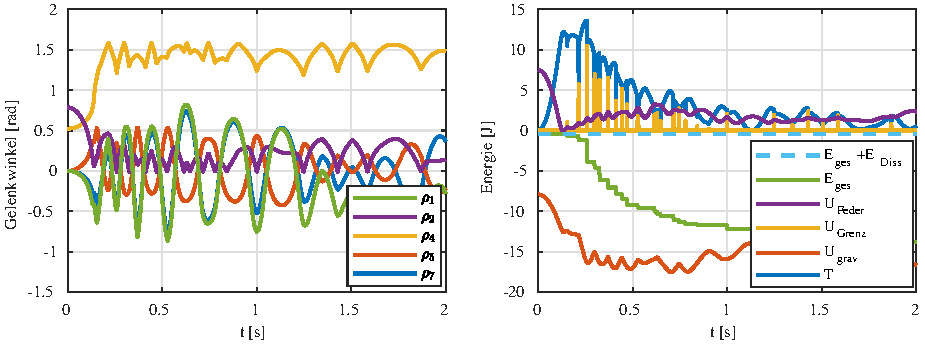
\includegraphics{figures/KAS5m5_Gelenkgrenzmodell_q_E.pdf} 
    \caption{variations in time of a simulation to check energy consistency. Left: Minimal coordinates from (\ref{equ:mincoord}). Right: Energies (kinetic $T$, gravity $U_\mathrm{g}$, elasticity of modeled joint limits $U_\mathrm{limit}$, linear spring $U_\mathrm{s}$, total energy $E_\mathrm{total}$, Dissipated energy $E_\mathrm{Diss}$). TODO: Regenerate figure with new colours and legends.}
    \label{fig:SimulationEnergiekonsistenz}
\end{figure*} 
%
Further, the results were compared and validated against a SimMechanics model of the mechanism.

This simulation is extended by the use of a human upper body musculoskeletal model, coupled with an elasticity to the tool handle of the exoskeleton via the term $\bm{\tau}_{1\mathrm{ext}}$ in (\ref{equ:ForwDyn}), which is elaborated in \cite{KuehnHuSchHad2018}.
%This allows to ...

\subsection{Computation}

The inverse dynamics (\ref{equ:Dyn_MinKoord}) of the constrained system was derived using the different approaches presented in this paper.
The computational effort to compute the terms of the dynamics is compared in Tab.\,\ref{tab:computation}.
The methods are 
%
\begin{enumerate}
    \item \emph{Trigonometric elimination} of the constraints by substituting with (\ref{equ:kinconstr_semiexplicit_sin})-(\ref{equ:kinconstr_semiexplicit_cos}) as described in Sec.\,\ref{sec:Lagrange2Elim}, 
    \item \emph{Direct elimination} of the constraints by directly using (\ref{equ:kinconstr_explicit}) to substitute the dependent joint coordinates in (\ref{equ:Lagrange_energy}),
    \item using \emph{implicit constraint equations} as described in Sec.\,\ref{sec:DynamicsImpl}.
\end{enumerate}
%
The expressions are generated with Maple using the procedure \texttt{optimize(tryhard)} and the number of operations is counted with the procedure \texttt{cost}.
%
\begin{table}
    \caption{Comparison of the computational effort for different implementations of the inverse dynamics.}\par\vspace{-3ex}
    \label{tab:computation}
    \centering
    \setlength\tabcolsep{3pt}
    \begin{tabular}[t]{|c|c|c|c|c|c|c|}
        \hline
        Method & Add. & Mult. & Fcn & Ass. & Sum & $t_\mathrm{Gen}$ [s] \\
        \hline
        \rowcolor{Gray}
        1: Trig. elim.  & 710 & 997 & 28 & 365 & \textbf{2100} & 4934 \\
        \rowcolor{Gray}
        2: Direct elim. & 674 & 937 & 43 & 358 & \textbf{2012} & 6510 \\
        $\bm{W}$ & 40 & 72 & 22 & 36 & 170 & 1 \\
        $\bm{g}$ & 474 & 609 & 28 & 235 & 1346 & 1 \\
        \rowcolor{Gray}
        3: Implicit constr. & 514 & 681 & 50 & 271 & \textbf{1516} & 2 \\
        \hline
    \end{tabular}
\end{table}
%

Since the results are qualitatively similar for different categories, additions (``Add.''), multiplications and divisions (``Mult.''), function calls to trigonometric and square root functions (``Fcn.'') and assignments of temporary variables (``Ass.'') are summed up.
The time for computation depends on the concrete hard- and software.\added[id=Lg,remark={Methode 2 hat die wenigstens Funktionsaufrufe, die sehr viel teurer als Add oder Ass sind. Die Zeit wäre hier schon interessant. Vllt. gibt es Literatur, in der Faktoren für verschiedenen Operatoren zu finden sind.
Beispiel: {http://www.latkin.org/blog/2014/11/09/a-simple-benchmark-of-various-math-operations/}
}]{}

Since the inverse dynamics of the open loop tree structure can be calculated very efficiently and the sparsity of the projection matrix $\bm{W}$ is high, benefiting the symbolic inversion, the standard method 3 has an about 25\,\% lower computational effort compared to the methods 1 and 2.
These methods based on elimination perform similar regarding the operation count.
The time needed to optimize and generate the code is about 25\,\% lower for the proposed method 3, indicating that the computer algebra system does not perform well for the kind of expressions produced in method 2.

%Using method 1 needs more multiplications and additions probably due to the products in the angle sum identities.

\section{Conclusions and future work}
\label{sec:conclusion}

%conclusion:
We presented a novel concept for a force assistance exoskeleton to support workers in carrying and using powertools.
The details of the solution of the kinematic constraints of the multi-loop mechanism focus on the elimination of trigonometric expressions of dependent variables.
This reduces the computational load when creating symbolic code for the terms of the dynamics equation with a similar efficiency of the output.
However, the presented approach does not reach the performance of the standard solution.

%Future work:
The featured approach of implementing kinematic constraints will be applied to different serial-chain industrial robots with parallel mechanisms invoking kinematic constraints, i.\,e. hybrid robots. 
The results will be compared to the classical approach using the projection of constraint forces and with non-trigonometric elimination of the constraints.

%\addtolength{\textheight}{-1cm}   % This command serves to balance the column lengths
                                  % on the last page of the document manually. It shortens
                                  % the textheight of the last page by a suitable amount.
                                  % This command does not take effect until the next page
                                  % so it should come on the page before the last. Make
                                  % sure that you do not shorten the textheight too much.

%%%%%%%%%%%%%%%%%%%%%%%%%%%%%%%%%%%%%%%%%%%%%%%%%%%%%%%%%%%%%%%%%%%%%%%%%%%%%%%%



%%%%%%%%%%%%%%%%%%%%%%%%%%%%%%%%%%%%%%%%%%%%%%%%%%%%%%%%%%%%%%%%%%%%%%%%%%%%%%%%



%%%%%%%%%%%%%%%%%%%%%%%%%%%%%%%%%%%%%%%%%%%%%%%%%%%%%%%%%%%%%%%%%%%%%%%%%%%%%%%%
%\section*{APPENDIX}
%
%Appendixes should appear before the acknowledgment.


%\section*{ACKNOWLEDGMENT}


%%%%%%%%%%%%%%%%%%%%%%%%%%%%%%%%%%%%%%%%%%%%%%%%%%%%%%%%%%%%%%%%%%%%%%%%%%%%%%%%


% BIBLIOGRAPHY
\bibliographystyle{ieeetr}
\bibliography{ref}
\end{document}
\grid
